\label{chapter:resultados}

Este capítulo tem como objetivo apresentar o planejamento, execução e análise dos resultados obtidos a partir implementação do método proposto no sistema Hand.io. Esta avaliação teve como foco funcionamento do protótipo da luva por meio de um experimento em um cenário real levando em consideração a eficácia e a eficiência do sistema em situações de utilização nominal.

\section{Análise da implementação}

Nesta seção é detalhado e analisado de maneira extensiva as particularidades da implementação da Hand.io, tanto no projeto do \textit{hardware} quanto de \textit{software}.
% 
% \subsection{Análise do protótipo}
% 
Como havia sido definido anteriormente no método proposto no \autoref{chapter:metodo}, o protótipo da Hand.io consiste em duas partes, a luva de captura de movimentos e a central de processamento de sinais que controla de dispositivos que serão analisados de forma individual.

\subsection{Protótipo da luva de captura de movimentos}

A luva é composta por três principais componentes: 
(\ref{fig:dorso}) microcontrolador Arduino UNO, que decodifica os sinais do sensor e os envia pela porta serial conectada à central de processamento; 
(\ref{fig:dorso}) um sensor MPU $6050$ que conta com um acelerômetro e um giroscópio, utilizado para realizar a leitura dos movimentos; e 
(\ref{fig:palma}) um botão, que é acionado pelo usuário para definir o início e o fim da captura dos movimentos. Os três componentes podem ser vistos na \autoref{fig:luva}.

\begin{figure}[ht]
    \centering
    \subfloat[\label{fig:dorso}]
        {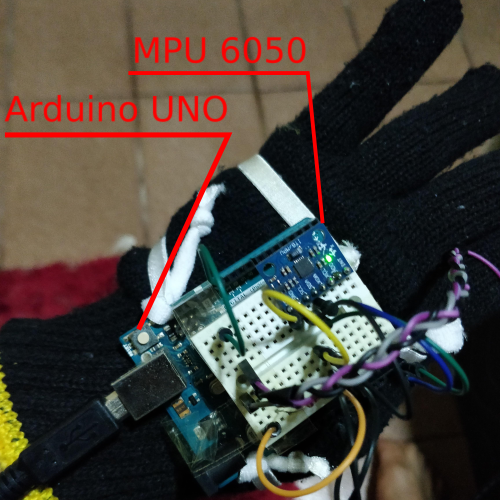
\includegraphics[width=0.4\textwidth]{resources/luva1.png}}
        \hspace{0.5cm}
    \subfloat[\label{fig:palma}]
        {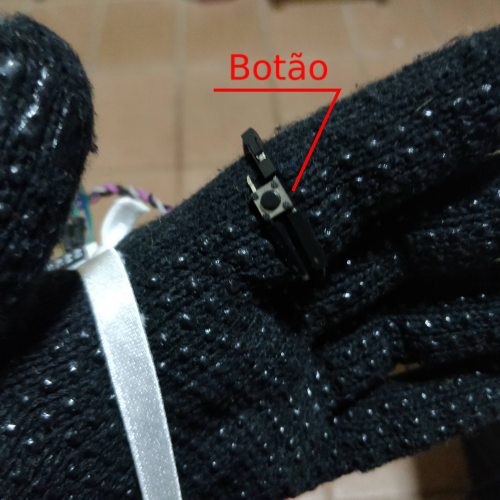
\includegraphics[width=0.4\textwidth]{resources/luva2.png}}
        \caption{Projeto da luva}
        \label{fig:luva}
\end{figure}

% Os componentes estão posicionados de maneira a garantir o máximo de conforto possível ao usuário. 
% É recomendada a utilização de 
Neste prototiopo foi adotada uma luva de pano para reduzir o contato do Arduino com a pele.
% , pois os pontos de solda no verso da placa podem criar eventuais escoriações com a utilização prolongada do sistema. 
O Arduino foi posicionado no dorso da mão, preso com fitas elásticas firmes para evitar movimentações indesejadas que levariam à uma leitura imprecisa dos movimentos.
% 
O sensor MPU $6050$ está fixado em uma \textit{mini protoboard} presa no topo do Arduino com fitas adesivas de maneira estável. O botão de acionamento de captura de movimentos conta com os seus fios trançados a fim aumentar a rigidez da construção do protótipo. Ao final da trança os fios são ligados ao botão de modo a formar um anel em volta do dedo indicador do usuário. Este posicionamento visa aumentar a ergonomia da luva, pois o botão estará convenientemente localizado no alcance do polegar do operador.

\subsection{Protótipo da central de processamento de sinais}

O esquemático da central apresentado na \autoref{fig:esq_central} do \autoref{chapter:metodo} define que a central é composta por um computador de propósito geral equipado com um microprocessador, capaz de executar algoritmos de aprendizado de máquina e enviar e receber sinais infravermelhos. Componentes com as mesmas funcionalidades dos propostos anteriormente foram utilizados no protótipo final, de maneira que foi possível validar o método proposto sem que fossem realizadas mudanças significativas.

\begin{figure}[ht]
    \centering
    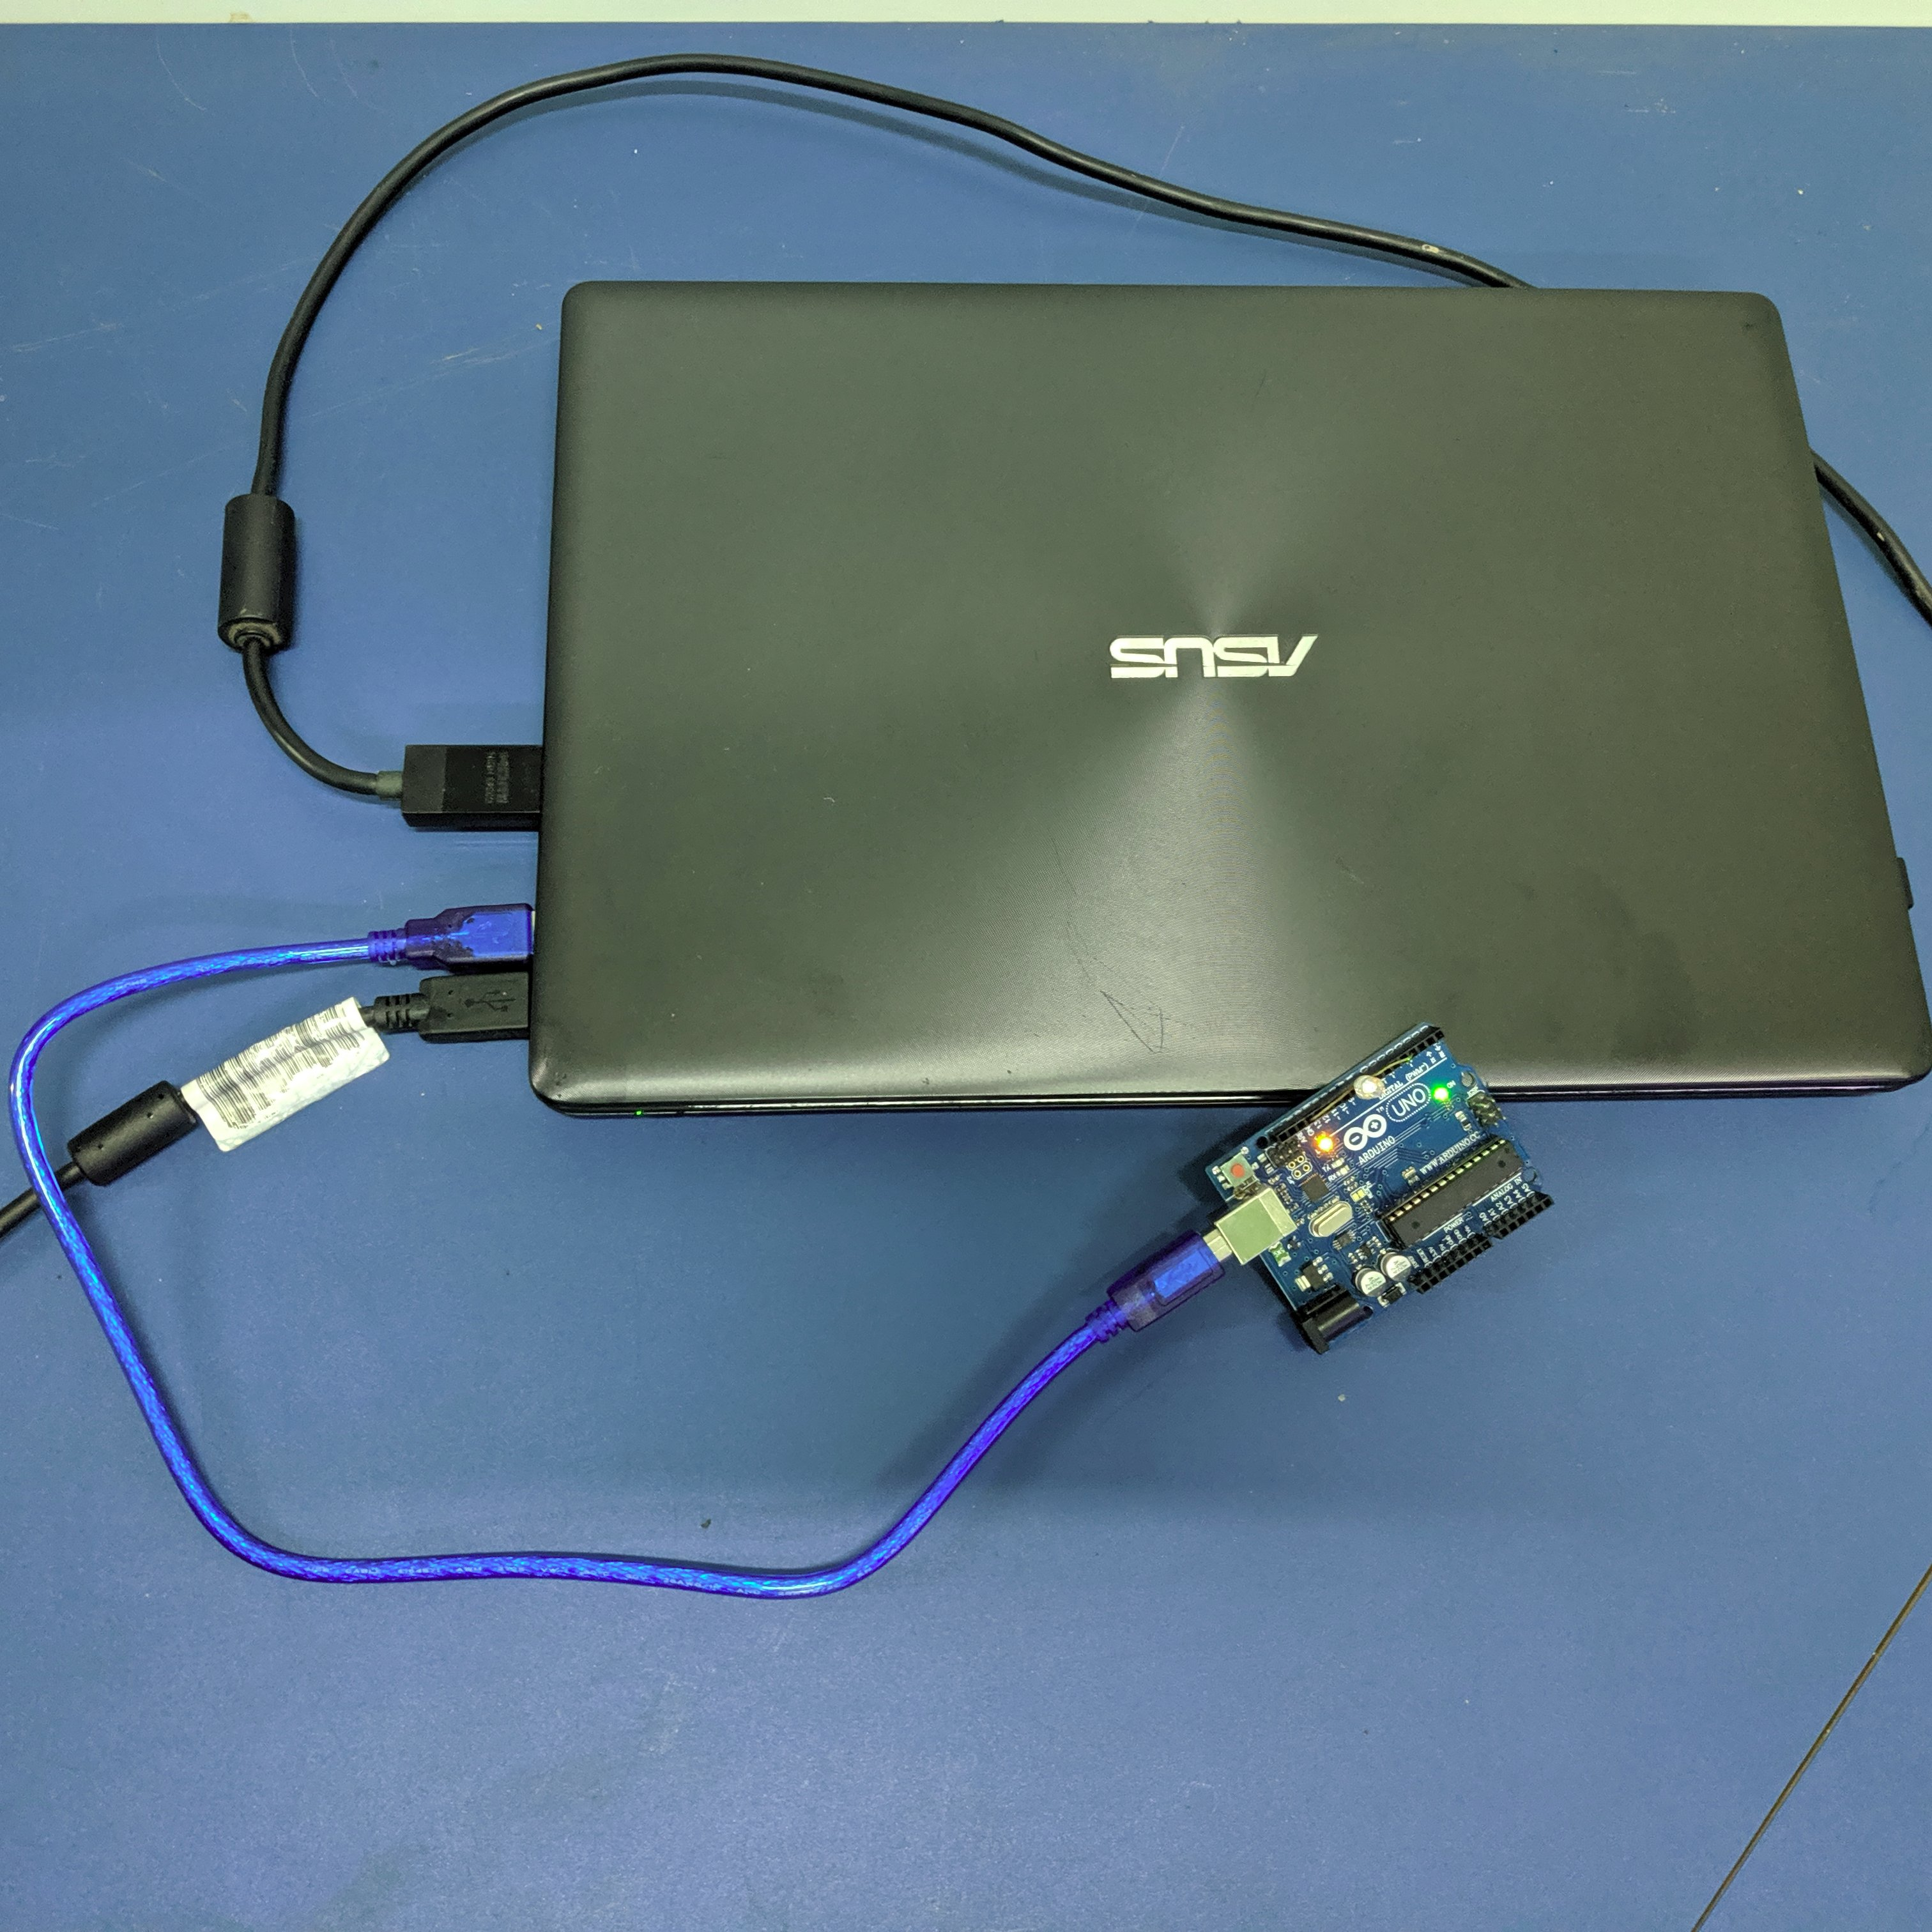
\includegraphics[width=0.5\textwidth, keepaspectratio]{resources/central.jpg}
    \caption{Central de controle}
    \label{fig:central}
\end{figure}

O protótipo da central exibido na \autoref{fig:central}, é composto por um Notebook Asus com um processador \textit{Intel Core I5}, $6GB$ de memória \textit{RAM}, rodando o sistema operacional Manjaro Linux 18.0.4, conectado à luva através de uma conexão serial via cabo por uma porta USB, que processa os sinais recebidos e executa as ações correspondentes. Através de uma outra porta USB do Notebook, uma outra conexão serial ligada à um segundo Arduino UNO, que atua como atuador, é realizada. Este Arduino faz o papel de receptor e emissor de sinais infravermelhos para o controle de dispositivos no ambiente. 
% É recomendado que o atuador fique em um lugar próximo aos dispositivos que se deseja controlar devido ao alcance limitado do emissor de infravermelho.



\subsection{Análise do software do protótipo}

Existem três softwares sendo executados simultaneamente de maneira independente no protótipo. Um no Arduino acoplado à luva, um no Arduino conectado à central e um na central. O código-fonte deste projeto está disponível no repositório online GitHub \url{https://github.com/JohnPinto/Hand.io}.

\subsubsection{Análise do software dos Arduinos}

Os softwares em execução nos dois Arduinos funcionam de maneira distinta. Durante a modelagem do sistema, foi definido que o Arduino presente na luva funcionaria apenas como sensor, enviando os sinais dos movimentos para a central,  enquanto o encontrado na central serviria de atuador, enviando os sinais infravermelhos para os dispositivos a serem controlados.

No decorrer do funcionamento nominal do sistema o Arduíno embutido na luva lê os sinais do sensor em tempo real. Enquanto o botão de captura de movimentos presente na luva não for pressionado pelo usuário, é enviado para a central apenas uma sequência de pontos (\texttt{.}) com um curtíssimo intervalo de tempo entre os envios. 

O comportamento de envio intercalado de pontos (\texttt{.}) e sinais de movimento serve de condição de marca parada para o classificador de movimentos encontrado na central que será detalhado nas seções a seguir. Foi utilizada a biblioteca \textit{SoftwareSerial}\footnote{\url{https://www.arduino.cc/en/Reference/SoftwareSerial}\label{ftnote:serial}} para a realização de comunicação serial.

Quando o botão é pressionado, a luva passa a enviar, pela porta serial, o sinal do acelerômetro e do giroscópio formatado  seguindo o padrão \texttt{\$    ax    ay    az    gx    gy    gz    $\setminus $n}, onde as componentes \texttt{x, y} e \texttt{z} dos sensores são indicadas pela letra \texttt{a} para acelerômetro e \texttt{g} para giroscópio, o \texttt{\$}, indica o início da leitura e o \texttt{$\setminus $n}, uma quebra de linha, indica o fim. 

% O sinal é enviado desta maneira afim de garantir a consistência da transmissão dos dados. 

O Arduino conectado à central que serve de atuador, permanece ocioso até que um comando indicando qual sinal infravermelho deverá ser enviado seja recebido. Os códigos infravermelhos ficam armazenados diretamente no Arduino, graças ao desacoplamento dos códigos da memória RAM para a flash\footnote{\url{https://www.arduino.cc/reference/en/language/variables/utilities/progmem/}}, isto permite ao usuário realizar o cadastro de centenas de códigos infravermelhos de dispositivos diferentes. 

Devido à natureza estacionária da central, é possível que múltiplos atuadores estejam inseridos em diversos cômodos diferentes de uma casa, por exemplo, o que serviria de aplicação para este trabalho. Na implementação deste software foram utilizadas as biblioteca SoftwareSerial\textsuperscript{\ref{ftnote:serial}}, para comunicação serial, e IRremote\footnote{\url{https://github.com/z3t0/Arduino-IRremote}}, para envio de sinais infravermelhos a partir do Arduino.


\subsubsection{Análise do software da central}


O softwares em execução na central de processamento tem a implementação detalhada na \autoref{fig:class}, onde é apresentado o diagrama de classes que define as especificidades do sistema e detalha as relações entre as classes que o constituem.

\begin{figure}[ht]
    \centering
    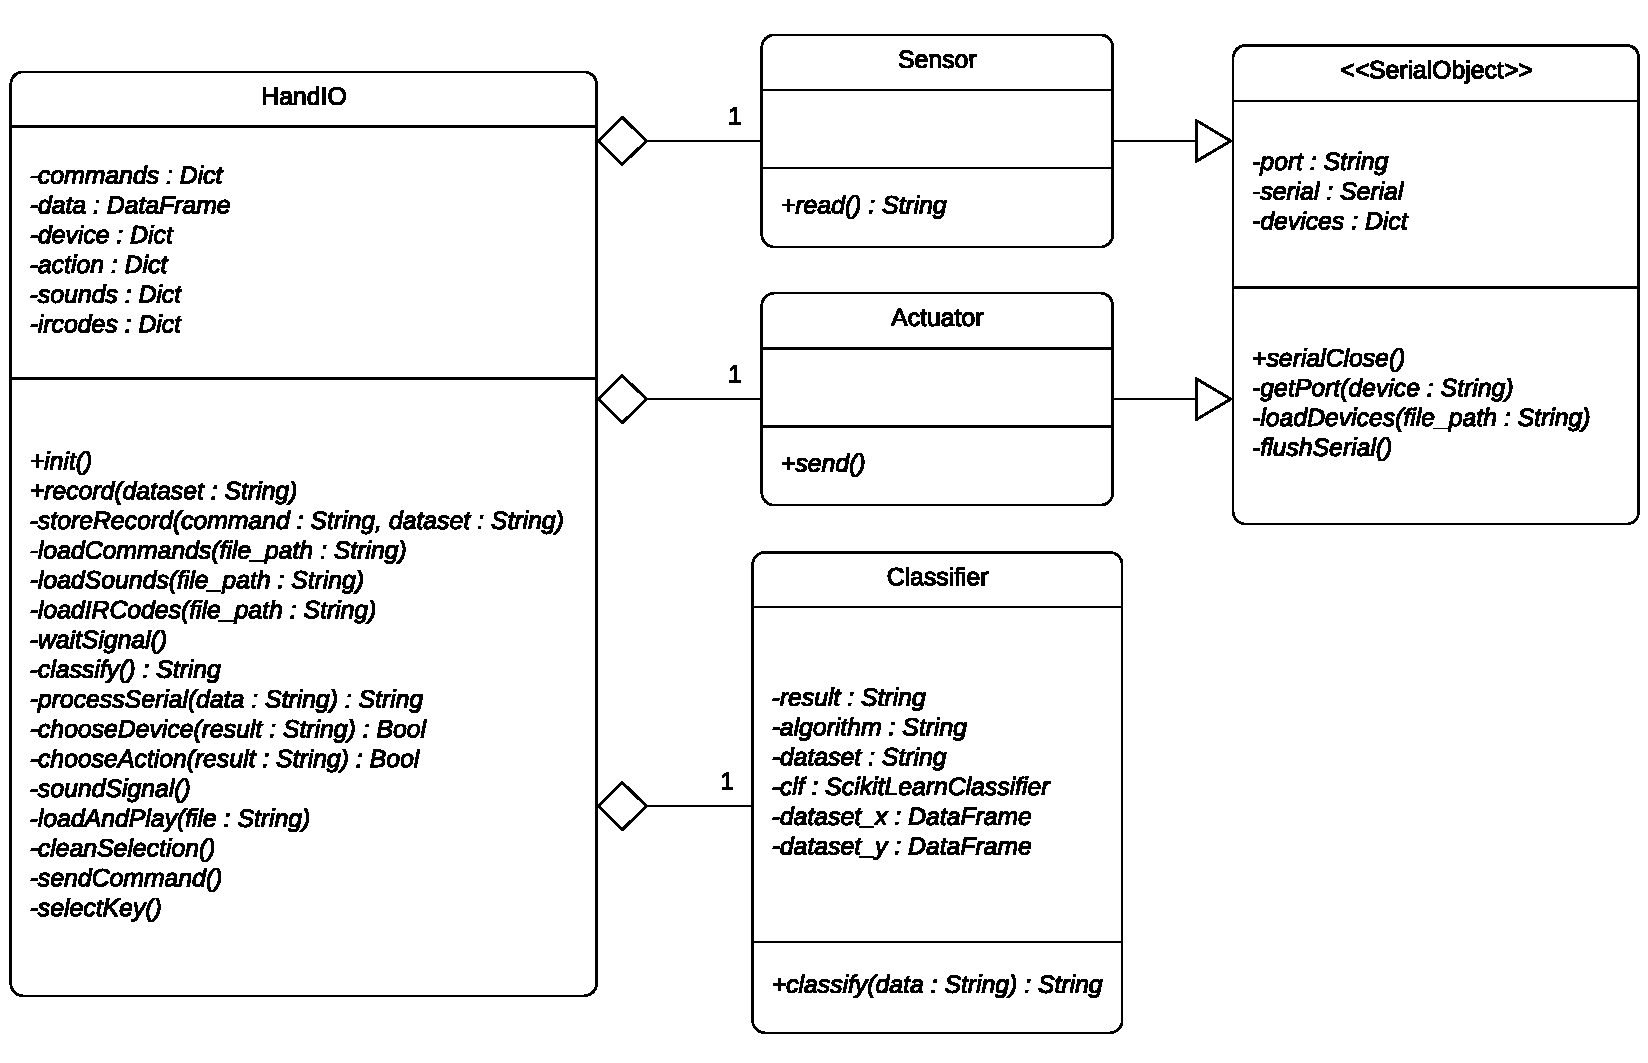
\includegraphics[width=\textwidth, keepaspectratio]{resources/diagrama_classe.pdf}
    \caption{Diagrama de classe da Hand.io}
    \label{fig:class}
\end{figure}

O código-fonte foi desenvolvido na linguagem de programação Python $3$, utilizando conceitos de programação orientada a objetos, como classes e herança, visando compartimentalizar o código com o objetivo de aumentar a previsibilidade, e evitar retrabalhos por parte do desenvolvedor. 

A linguagem em questão foi escolhida por sua praticidade de implementação graças à sua natureza de alto nível, o que permite uma implementação rápida e simples em comparação com as demais linguagens. Outro grande fator motivador é a presença de uma vasta gama de bibliotecas externas que agilizaram grandemente o desenvolvimento do protótipo, como o Scikit-learn\footnote{\url{https://scikit-learn.org/}\label{ftnote:sklearn}}, que dispõe de biblioteca Scikit-learn que conta com uma série de classificadores que utilizam algoritmos de aprendizado de máquina já implementados, e a PySerial\footnote{\url{https://github.com/pyserial/pyserial}\label{ftnote:pyserial}} que reliza o interfaceamento entre a linguagem Python e a porta serial do sistema.

No diagrama de classes da \autoref{fig:class} a \texttt{HandIO} é a classe principal do sistema. Esta classe conta com definições de sensor, atuador e classificador. Ambos os sensores e atuadores, implementados nas classes de nomes correspondentes, herdam da classe abstrata \texttt{SerialObject}, com a diferença de que o sensor tem a capacidade de enviar sinais e o atuador apenas de recebe-los. Internamente a classe \texttt{SerialObject} utiliza a biblioteca PySerial, para a transmissão de dados. 

A classe \texttt{HandIO} conta com diversos dicionários que agem como um especie de banco de dados do sistema, esta abordagem foi escolhida para que haja a possibilidade do desenvolvedor do sistema modificar ou adicionar novos gestos ou dispositivos de maneira simplificada. Todos os dicionários utilizados são carregados a partir de seus arquivos \texttt{.json} correspondentes que podem ser encontrados na pasta \texttt{json/} da raiz do sistema. Foram implementados métodos privados que iniciam com a palavra \texttt{load}, que carregam cada dicionário individualmente, estes métodos são chamados no construtor do objeto.

O classificador, implementado na classe \texttt{Classifier}, utiliza a biblioteca Scikit-learn. Esta biblioteca foi escolhida por suprir as necessidades do protótipo e contar com uma \texttt{API} de utilização bastante simplificada. Os \textit{datasets} com registros de movimentos utilizados para geração do modelo de classificação dos gestos ficam armazenados na pasta \texttt{datasets/} do programa. 

A geração destes \textit{datasets} se dá utilizando o método público \texttt{record()} da classe \texttt{HandIO}, que pede que o usuário da luva insira uma classe, que define qual gesto será registrado, e realize $10$ gestos. Este procedimento se repete até que o usuário pare o programa. Para o protótipo foi levantado um \texttt{dataset} com $360$ leituras recolhidas de nove voluntários diferentes, distribuídas entre quatro classes de gestos correspondentes à movimentos nas direções cima, baixo, direita e esquerda. Os voluntários foram orientados a realizarem os gestos com a palma da mão voltada para a direita. Estes gestos foram escolhidos devido ao seu baixo grau de complexidade o que facilitaria os experimentos detalhados nas seções seguintes.

Para a definição de qual classificador seria o mais eficaz para a classificação de gestos, foi realizado um comparativo, com os principais classificadores oferecidos pela biblioteca Scikit-learn, sendo estes: a \textit{Logistic Regression} (LR), a \textit{Linear Discriminant Analysis} (LDA), o \textit{K-Neighbors Classifier} (KNN), o \textit{Decision Tree Classifier} (CART), a \textit{Gaussian Naive Bayes} (NB), a \textit{Suport Vector Machine} (SVM), o \textit{Ada Boost Classifier} (ADB), o \textit{Random Forest Classifier} (RFC), o \textit{Extra Trees Classifier} (ETC), e o \textit{Gradient Boosting Classifier} (GBC).

Este comparativo foi realizado utilizando validação cruzada, que é uma técnica que divide o \textit{dataset} em grupos de treinamento e grupos de teste. O grupo de treinamento é utilizado para a criação do modelo de classificação que serve de referência para classificações futuras, e o grupo de testes é utilizado como entrada para o classificador, esperando que a classificação seja bem sucedida, já que ambas as partes fazem parte de um mesmo \textit{dataset}. Para uma medição mais precisa foi utilizada a técnica conhecida como \textit{K-fold}, que realiza $K$ testes de validação cruzada pegando $K$ partes diferentes do \textit{dataset} como treinamento e teste a cada $K$ interações. Para a obtenção de resultados consistentes foi utilizado um $K = 10$.

Os resultados constatados na \autoref{fig:classificadores} indicam que o classificador com melhor desempenho foi o \textit{Gaussian Naive Bayes} (NB), que obteve uma acurácia de 81.1\% durante a validação cruzada, sem que tenha havido uma perda considerável na pontuação de treino no decorrer do aumento da quantidade de registros de movimento no \textit{dataset}. 

\begin{figure}[ht]
    \centering
    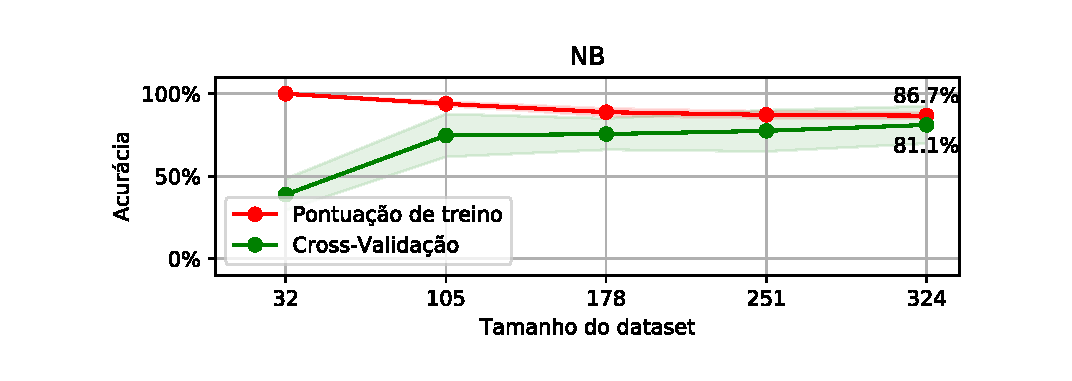
\includegraphics[width=0.8\textwidth, keepaspectratio]{resources/comparacao.pdf}
    \caption{Resultados da comparação de classificadores}
    \label{fig:classificadores}
\end{figure}

Apesar do gráfico do NB com 32 valores valores no \textit{dataset} ter atingido uma pontuação de treino alta em relação à uma quantidade maior, o modelo gerado com apenas esta quantidade de valores não é genérico o suficiente para classificar os movimentos de um segundo usuário com precisão, por isso é necessária uma quantidade maior de leituras realizadas por usuários diferentes, o que justifica a escolha deste classificador como o classificador padrão deste sistema.

\subsection{Fluxo de execução}

O sistema conta com duas grandes fases apresentadas na máquina de estados da \autoref{fig:automato}. A fase de seleção de dispositivo, definida na parte superior da figura, e a fase de seleção de ação, na parte inferior. O fluxo de execução será abordado do ponto de vista da máquina de estados, realizando anotações sobre quais métodos das classes, expostos na \autoref{fig:class}, são chamados durante um dado estado. 
% 
Na classe \texttt{HandIO} está implementado o método público \texttt{init()}, que é responsável pelo funcionamento nominal da central. Os procedimentos dentro deste método, refletem o comportamento definido na máquina de estados apresentada anteriormente.

\begin{figure}[ht]
    \centering
    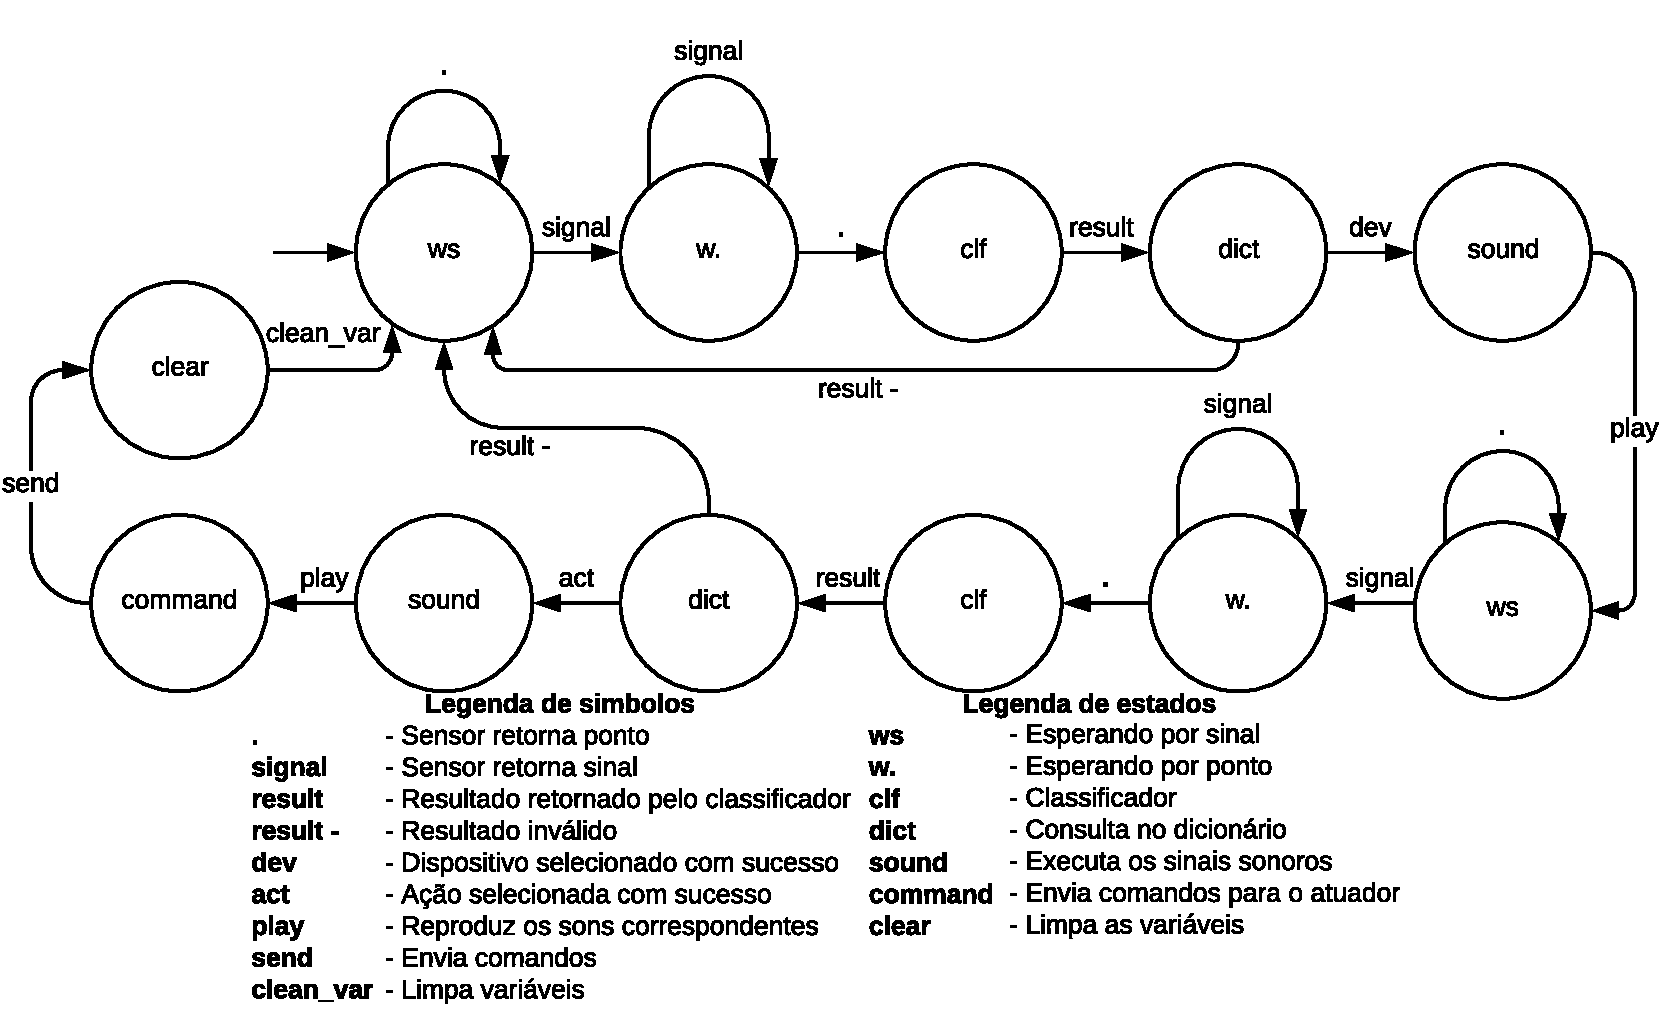
\includegraphics[width=\textwidth, keepaspectratio]{resources/maquina_estados.pdf}
    \caption{Máquina de estados da Hand.io}
    \label{fig:automato}
\end{figure}

Durante os estágios iniciais da primeira e da segunda fase, os estados \textbf{ws} e \textbf{w.}, que foram implementados no método \texttt{waitSignal()}, o sistema fica aguardando os sinais de início e parada de captura de movimentos. Em um primeiro momento que forem recebidos pontos pela serial, a central permanece no estado \textbf{ws}, ao ser constatado o recebimento de um sinal de movimento, o sistema passará para o estado \textbf{w.}.

O programa permanecerá neste estado até que voltem a ser recebidos pontos, para que então o ultimo sinal recebido seja salvo no atributo \texttt{data}, e enviado para o classificador no estado \textbf{clf} que chama o método \texttt{classify()}. Após o retorno da classificação, o sistema passará para o estado \textbf{dict}, onde os resultados serão avaliados.

Neste estado o resultado da classificação serve como entrada para o método \texttt{chooseDevice()} ou para o método \texttt{chooseAction()}, dependendo da fase que o programa se encontra. Nestes métodos o resultado é utilizado como chave no dicionario \textit{commands} que retorna o dispositivo ou ação correspondente ao gesto. 
Caso o dicionário retorne um sinal válido o sistema então passa para o estado \textbf{sound}, que chama o método \texttt{soundSignal()} caso o retorno seja inválido o sistema retornará ao estado inicial. Durante a segunda fase do programa os possíveis retornos do dicionário ficam restritos às possíveis ações que dispositivo previamente selecionado tem mapeados pelo sistema. 

O estado \textbf{command}, implementado no método \texttt{sendCommand()}, analisa a ação selecionada no estado anterior e as realiza no dispositivo selecionado. Ao final das duas fases o sistema entra no estado \textbf{clear}, que limpa a seleção de dispositivo e gesto, para que um novo comando seja realizado. 

\section{Planejamento e projeto do cenário experimental}

\todo[inline]{Finalizar ASAP}

Um cenário no qual serão realizados os experimentos foi criado para avaliar a capacidade da Hand.io de controlar dispositivos em um ambiente real. Será utilizado nesta avaliação o protótipo discutido na seção anterior deste capítulo. Como referência do progresso dos experimentos, as questões experimentais levantadas abaixo serão respondidas conforme o andamento dos experimentos:

\begin{description}
    \item [QE1] \label{qa:1} Qual a taxa de sucesso do sistema em detectar os gestos corretamente e enviar sinais aos dispositivos correspondentes?
    \item [QE2] \label{qa:2} Um novo usuário que recebeu um roteiro simples de utilização da luva, consegue controlar os dispositivos do ambiente sem maiores dificuldades?
    \item [QE3] \label{qa:3} Qual a avaliação de um novo usuário sobre o estado atual do sistema?
\end{description}

O cenário experimental, apresentado na \autoref{fig:cenario}, conta com um ar-condicionado, do fabricante Carrier, uma TV da marca Philips e uma apresentação de slides que ocorre no \textit{notebook}, que serve de central para o sistema, e é exibida na TV. Para controle de dispositivos que contam com uma interface de controle por meio de sinais infravermelhos, como é o caso do ar-condicionado e da TV selecionas, é necessário que os sinais enviados pelos controles remotos destes dispositivos sejam capturados e carregados no Arduino que serve como atuador. Para controle da apresentação de slides, não é necessária intervenção por parte do instalador do sistema, pois o sistema já conta com as funcionalidades para este tipo de operação.

Foram realizados três experimentos, medindo a eficácia do sistema de maneiras diferentes. Com a finalidade de responder a primeira questão experimental (QE1), foi realizado um primeiro experimento onde um voluntário, que teve os seus dados de movimentos previamente cadastrados no sistema, reproduziu duas situações e teve a sua taxa de sucesso registrada quantitativamente.

Para a constatação da resposta da segunda questão experimental (QE2), um grupo voluntários, que nunca utilizaram o sistema e não tiveram seus dados de movimentos previamente registrados, foi instruído a seguir um roteiro escrito e teve a sua taxa de sucesso registrada para avaliação posterior. 

Este mesmo grupo a fim de responder a terceira questão experimental (QE3), após a execução do roteiro, participou de um questionário no qual são realizadas diversas perguntas sobre o estado atual do sistema, e quais possíveis melhorias poderiam ser feitas para melhorar a ergonomia do sistema a partir do ponto de vista de um eventual usuário final.

\begin{figure}[ht]
    \centering
    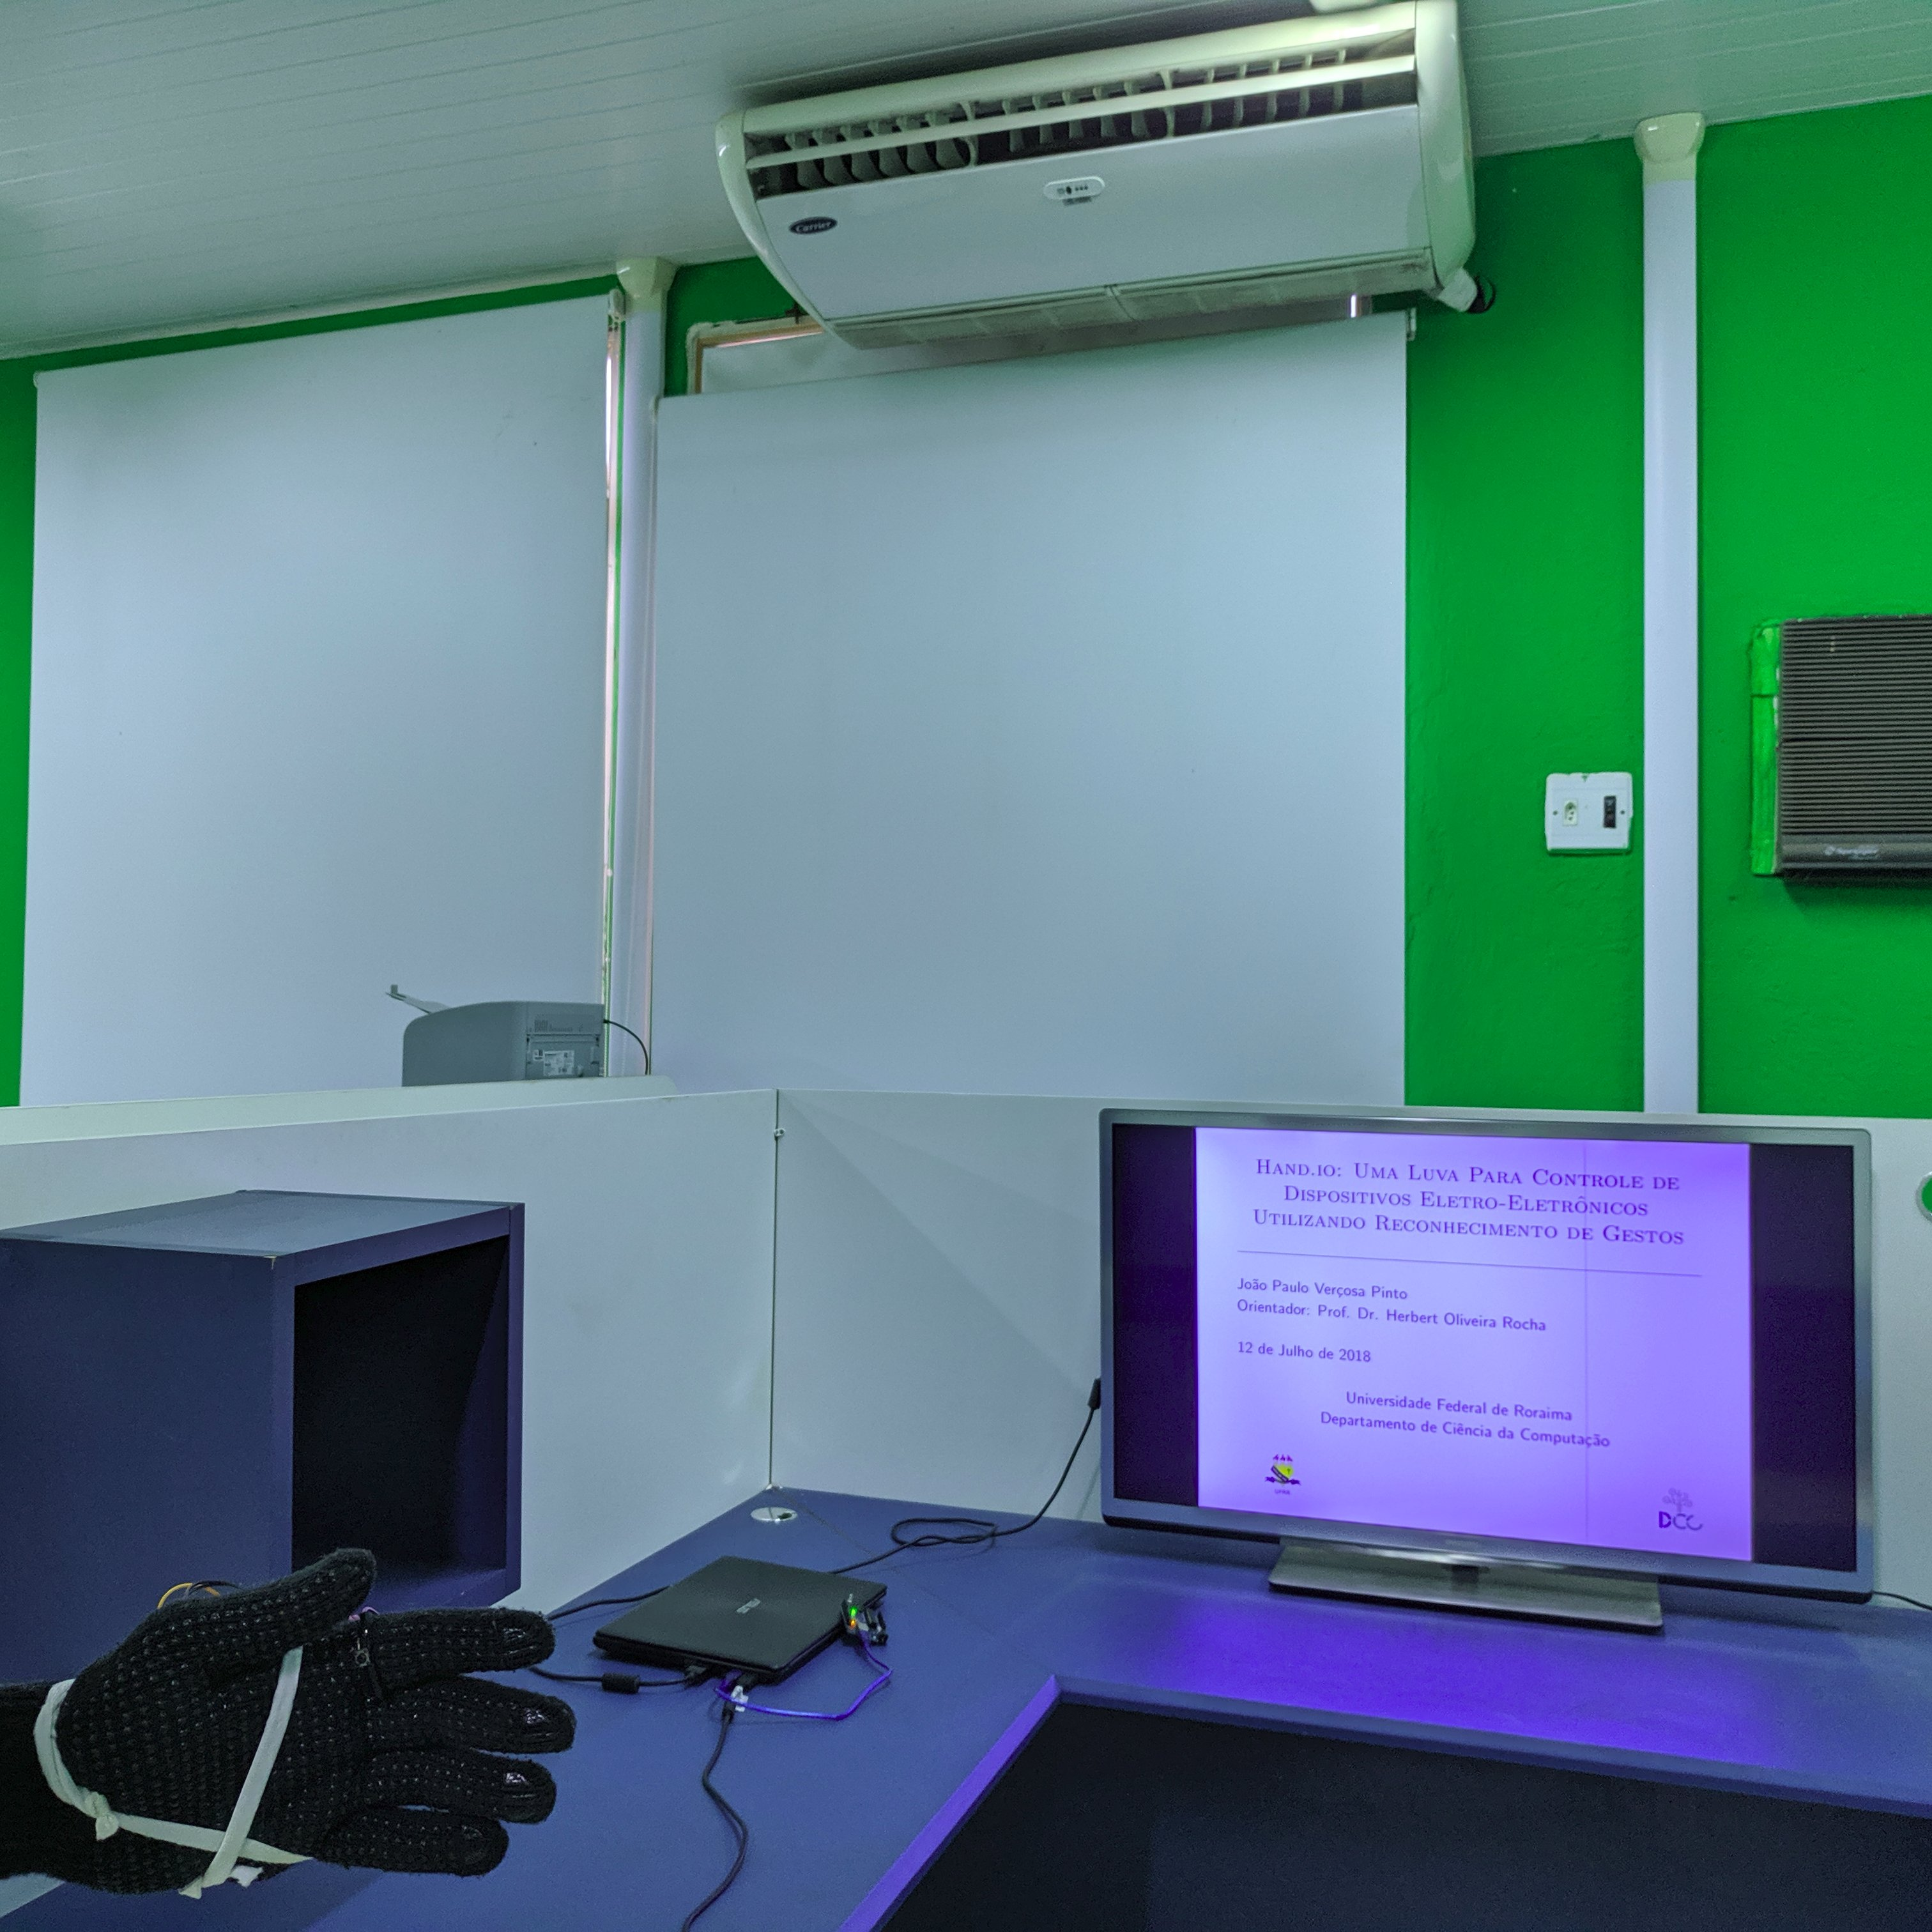
\includegraphics[width=0.5\textwidth, keepaspectratio]{resources/cenario.jpg}
    \caption{Cenário experimental}
    \label{fig:cenario}
\end{figure}


%\newpage

\section{Execução dos experimentos e análise dos resultados}

\subsection{Teste quantitativo com um usuário experiente}

Após a execução do primeiro experimento, os resultados foram registrados e estão expostos na \autoref{tab:resultados}, onde a primeira coluna representa o número do experimento, e a segunda, e terceira denotam os resultados das situações 1 e 2, respectivamente. Na situação 1 o usuário foi instruído a ligar e desligar sequencialmente a TV e o ar-condicionado presentes no cenário experimental. Já na situação 2 o usuário foi instruído a avançar ou retroceder a apresentação de slides reproduzida na TV. Cada resultado de um experimento $n$ está assinalado com um (OK) para bem sucedido e (F) para mal sucedido. 

A partir do total de 60 experimentos, distribuídos entre as situações 1 e 2, foi encontrada uma taxa média de sucesso de 93.3\%, o que demonstra de maneira evidente a eficácia do sistema. Apesar da taxa de falha ter sido pequena, ela não é desprezível em um sistema desenhado para um usuário final, logo se faz necessário um aprimoramento do classificador a fim de reduzir ainda mais esse percentual. Os resultados apresentados por este experimentos servem de resposta para a questão experimental 1 (\textbf{QE1}).

\begin{table}[ht]
    \centering
    \begin{tabular}{c|c|c|c|c|c|c|}
        \cline{2-7}
        & \multicolumn{4}{c|}{\textbf{Situação 1}} & \multicolumn{2}{c|}{\textbf{Situação 2}} \\ 
        \hline
        \multicolumn{1}{|c|}{$n$} & \textbf{Ligar TV} & \textbf{Ligar AC} & \textbf{Desligar TV} & \textbf{Desligar AC} & $\rightarrow$ & $\leftarrow$ \\
        \hline
        \multicolumn{1}{|c|}{\textbf{1}}  & OK & OK & OK & OK & OK & OK \\ \hline
        \multicolumn{1}{|c|}{\textbf{2}}  & OK & OK & OK & OK & OK & OK \\ \hline
        \multicolumn{1}{|c|}{\textbf{3}}  & OK & OK & OK & OK & OK & OK \\ \hline
        \multicolumn{1}{|c|}{\textbf{4}}  & OK & OK & OK & OK & OK & OK \\ \hline
        \multicolumn{1}{|c|}{\textbf{5}}  & OK & OK & OK & OK & OK & OK \\ \hline
        \multicolumn{1}{|c|}{\textbf{6}}  & OK & OK & OK & F  & OK & OK \\ \hline
        \multicolumn{1}{|c|}{\textbf{7}}  & OK & F  & OK & OK & OK & F  \\ \hline
        \multicolumn{1}{|c|}{\textbf{8}}  & OK & OK & OK & OK & OK & OK \\ \hline
        \multicolumn{1}{|c|}{\textbf{9}}  & OK & F  & OK & OK & OK & OK \\ \hline
        \multicolumn{1}{|c|}{\textbf{10}} & OK & OK & OK & OK & OK & OK \\ \hline
        \multicolumn{1}{|c|}{\begin{tabular}[c]{@{}c@{}}\textbf{Taxa}\\\textbf{de sucesso}\end{tabular}} & $100\%$ & $80\%$ & $100\%$ & $90\%$ & $100\%$ & $90\%$ \\ \hline
        \multicolumn{7}{|c|}{\textbf{Taxa média de sucesso:} $93.3\%$} \\ \hline
    \end{tabular}
    \caption{Resultados do experimento 1}
    \label{tab:resultados}
\end{table}



%\newpage 

\subsection{Teste quantitativo com voluntários inexperientes}

Um grupo com cinco voluntário que não tiveram contato posterior com o sistema, foram instruídos a seguir um roteiro com a finalidade de avaliar a usabilidade e funcionamento da Hand.io. Os resultados deste experimento estão expostos na \autoref{tab:roteiro} abaixo, onde \textbf{V1}, \textbf{V2}, \textbf{V3}, \textbf{V4}, e \textbf{V5}, representam os voluntários. 

O roteiro é composto por 6 passos, onde no primeiro passo (\textbf{1}) se pediu que o ar-condicionado presente no cenário experimental fosse ligado, no segundo passo (\textbf{2}), os voluntários foram instruídos a ligar a TV, no terceiro passo (\textbf{3}), foi solicitado ao voluntários que fossem passados cinco slides em uma determinada apresentação, no passo quatro (\textbf{4}), se pediu que fossem voltados 2 slides da mesma apresentação do passo 3, no quinto passo (\textbf{5}) foi instruído que a TV fosse desligada e finalizando no passo seis (\textbf{6}) foi solicitado o desligamento do ar-condicionado.

Os resultados foram quantificados utilizando (OK) para bem sucedido, (P) para sucesso parcial, onde foi permitida uma tentativa para a realização do comando, mais que isso o resultado foi contabilizado como (F) falha. Quando houveram problemas durante a execução dos experimentos, o aplicador do experimento realizou anotações quanto à possível razão. Estas anotações estão representadas na \autoref{tab:roteiro}, nas notas de rodapé. 

Após a análise dos resultados deste experimento foi constatada uma taxa média de sucesso de $89.08\%$, nesta média foram considerados apenas os experimentos bem sucedidos. Apesar do desempenho ter sido inferior em relação ao experimento anterior, neste caso vale salientar que os voluntários não tiveram qualquer contato prévio com o sistema e não tiveram seus dados de movimentos inseridos no classificador, o que demonstra que o modelo obtido a partir do \textit{dataset} inicial, se mostra genérico o suficiente para ser utilizado por terceiros. Após esta análise podemos dizer que a questão experimental 2  (\textbf{QE2}), pode ser considerada como respondida.

\begin{table}[ht]
    \centering
    \begin{threeparttable}
        \centering
        \begin{tabular}{c|c|c|c|c|c|}
            \cline{2-6}
             & \textbf{V1} & \textbf{V2} & \textbf{V3} & \textbf{V4} & \textbf{V5} \\ \hline
            \multicolumn{1}{|c|}{\textbf{1}} & OK & OK & OK & OK & P\tnote{1} \\ \hline
            \multicolumn{1}{|c|}{\textbf{2}} & P\tnote{1} & OK & OK & OK & OK \\ \hline
            \multicolumn{1}{|c|}{\textbf{3.1}} & P\tnote{1} & OK & OK & OK\tnote{3} & OK \\ \hline
            \multicolumn{1}{|c|}{\textbf{3.2}} & OK & OK & OK & OK\tnote{3} & OK \\ \hline
            \multicolumn{1}{|c|}{\textbf{3.3}} & OK & OK & OK & OK\tnote{3} & OK \\ \hline
            \multicolumn{1}{|c|}{\textbf{3.4}} & OK & OK & OK & OK\tnote{3} & OK \\ \hline
            \multicolumn{1}{|c|}{\textbf{3.5}} & OK & OK & OK & OK\tnote{3} & F \\ \hline
            \multicolumn{1}{|c|}{\textbf{4.1}} & P & OK & OK & P & OK \\ \hline
            \multicolumn{1}{|c|}{\textbf{4.2}} & OK & OK & OK & OK & OK \\ \hline
            \multicolumn{1}{|c|}{\textbf{5}} & OK & OK\tnote{2} & OK & OK & OK \\ \hline
            \multicolumn{1}{|c|}{\textbf{6}} & OK & OK & OK & OK & OK \\ \hline
            \multicolumn{1}{|c|}{\begin{tabular}[c]{@{}c@{}}\textbf{Taxa}\\\textbf{de sucesso}\end{tabular}} & $72.7\%$ & $100\%$ & $100\%$ & $90.9\%$ & $81.8\%$ \\ \hline
            \multicolumn{6}{|c|}{\textbf{Taxa média de sucesso:} $89.08\%$} \\ \hline
        \end{tabular}
        \begin{tablenotes}
            \item[1] Problemas por falta de familiaridade com o sistema.
            \item[2] Dificuldade em lembrar dos gestos.
            \item[3] Problemas com o botão de acionamento de leitura.
        \end{tablenotes}
    \end{threeparttable}
    \caption{Dados coletados do experimento}
    \label{tab:roteiro}
\end{table}

%\newpage

\subsection{Aplicação do questionário ao grupo de voluntários}

Após a realização do experimento anterior o grupo de voluntários respondeu à um questionário que avalia o sistema como um todo. As perguntas realizadas podem ser vistas na lista abaixo:

\begin{description}[noitemsep]
    \item [Q1] O quão satisfeito você está quanto à eficácia do sistema? (de 0 a 10)
    \item [Q2] Como você avalia os gestos utilizados para controlar o ambiente?(de 0 a 10)
    \item [Q3] Qual o seu interesse em adquirir uma versão finalizada do sistema? (de 0 a 10)
    \item [Q4] O quê você acha poderia ser aprimorado no sistema?
\end{description}

As primeiras três perguntas \textbf{Q1}, \textbf{Q2}, e \textbf{Q3}, fazem uma análise quantitativa do sistema, já a \textbf{Q4} espera uma resposta mais subjetiva. Os resultados do questionário está expostos na \autoref{tab:questionario}.

\begin{table}[ht]
    \centering
    \begin{tabular}{c|c|c|c|c|c||c|}
        \cline{2-7}
         & \textbf{V1} & \textbf{V2} & \textbf{V3} & \textbf{V4} & \textbf{V5} & \textbf{Média} \\ \hline
        \multicolumn{1}{|c|}{\textbf{Q1}} & 10 & 10 & 10 & 10 & 9 & 9.8 \\ \hline
        \multicolumn{1}{|c|}{\textbf{Q2}} & 9 & 10 & 9 & 9 & 10 & 9.4 \\ \hline
        \multicolumn{1}{|c|}{\textbf{Q3}} & 10 & 10 & 10 & 10 & 10 & 10 \\ \hline
    \end{tabular}
    \caption{Dados coletados do questionário}
    \label{tab:questionario}
\end{table}

A média das respostas da primeira pergunta (\textbf{Q1}), de 9.8 aponta que o sistema em seu estado atual atende às expectativas dos usuários. Este resultado positivo fortalece a ideia proposta por este trabalho, que apesar de ser um protótipo já recebe avaliações positivas em relação ao seu funcionamento. Já a segunda pergunta (\textbf{Q2}) contou com uma média de resposta de 9.4, a menor entre as perguntas. 

Isso pode ser explicado pela falta de familiaridade dos voluntários em relação a sistemas de controle por movimentos, um problema que seria resolvido caso os voluntários tivessem mais tempo de uso do sistema, ou pela baixa variedade de gestos, isso significa que devem ser feitos mais testes quanto à definição dos gestos. As respostas da terceira pergunta (\textbf{Q3}) tiveram  média 10, a mais alta de todas. Isso demonstra que existe mercado para um eventual produto final que possa surgir a partir deste trabalho.  

A quarta pergunta (\textbf{Q4}) gerou respostas diferentes de cada voluntário, o primeiro voluntário respondeu que seria interessante que a luva deixasse de utiliza um botão para definir o inicio e o fim dos gestos e passe a utilizar uma leitura contínua dos movimentos. Esta é uma abordagem interessante no entanto o grau de complexidade em definir os momentos onde o usuário deseja realizar comandos é alto, talvez com um estudo mais aprofundado este tipo de funcionalidade possa ser possível, no entanto isso está fora do escopo deste trabalho. 

O segundo voluntário sugeriu que pudesse ser realizado mais de um gesto por dispositivo selecionado, isto é, ao selecionar a TV fosse possível ligar e mudar de canal sem precisar que a TV fosse selecionada novamente para a realização do comando de mudar de canal. Esta funcionalidade pode ser implementada no sistema, no entanto seria necessário que o desenvolvedor criasse uma solução simples para esta mecânica sem que a complexidade na utilização aumentasse.

Foi sugerido pelo terceiro voluntário que caso um dispositivo tivesse sido selecionado por acidente, houvesse a possibilidade do usuário retornar para a seção de seleção sem que um comando seja realizado. Assim como na sugestão do segundo voluntário é necessário que o desenvolvedor faça um levantamento de como implementar esta funcionalidade sem reduzir a eficácia do sistema.

A resposta dada pelo quarto voluntário sugere que fossem adicionados mais opções de gestos para que mais dispositivos possam ser controlados e mais comandos possam ser realizados. Na implementação atual do sistema isso já é possível, mas um aumento na quantidade de gestos poderia dificultar na memorização por parte do usuário de qual gesto realiza qual ação. Seria necessária a realização de um estudo afim de definir qual o número ideal de gestos poderiam ser inseridos sem que o usuário começasse a se confundir.

O quinto e último voluntário respondeu que era do interesse de um eventual usuário que fosse possível a personalização do sistema, através do remapeamento dos gestos com as ações. O sistema já permite este tipo de operação, no entanto não existe uma interface para que um usuário final possa realizar estas mudanças. Os arquivos que definem estas funcionalidades são externos, logo um programa externo executado em um outro dispositivo, como por exemplo um \textit{smartphone}, poderia sem maiores dificuldades realizar estas alterações, basta que uma interface de rede seja incluída na central.

As respostas recebidas neste questionário servem de guia para 